% Options for packages loaded elsewhere
\PassOptionsToPackage{unicode}{hyperref}
\PassOptionsToPackage{hyphens}{url}
%
\documentclass[
  landscape]{article}
\usepackage{lmodern}
\usepackage{amssymb,amsmath}
\usepackage{ifxetex,ifluatex}
\ifnum 0\ifxetex 1\fi\ifluatex 1\fi=0 % if pdftex
  \usepackage[T1]{fontenc}
  \usepackage[utf8]{inputenc}
  \usepackage{textcomp} % provide euro and other symbols
\else % if luatex or xetex
  \usepackage{unicode-math}
  \defaultfontfeatures{Scale=MatchLowercase}
  \defaultfontfeatures[\rmfamily]{Ligatures=TeX,Scale=1}
\fi
% Use upquote if available, for straight quotes in verbatim environments
\IfFileExists{upquote.sty}{\usepackage{upquote}}{}
\IfFileExists{microtype.sty}{% use microtype if available
  \usepackage[]{microtype}
  \UseMicrotypeSet[protrusion]{basicmath} % disable protrusion for tt fonts
}{}
\makeatletter
\@ifundefined{KOMAClassName}{% if non-KOMA class
  \IfFileExists{parskip.sty}{%
    \usepackage{parskip}
  }{% else
    \setlength{\parindent}{0pt}
    \setlength{\parskip}{6pt plus 2pt minus 1pt}}
}{% if KOMA class
  \KOMAoptions{parskip=half}}
\makeatother
\usepackage{xcolor}
\IfFileExists{xurl.sty}{\usepackage{xurl}}{} % add URL line breaks if available
\IfFileExists{bookmark.sty}{\usepackage{bookmark}}{\usepackage{hyperref}}
\hypersetup{
  pdftitle={Bebés en Toluca},
  pdfauthor={Jorge Salvador Ruiz Montaño},
  hidelinks,
  pdfcreator={LaTeX via pandoc}}
\urlstyle{same} % disable monospaced font for URLs
\usepackage[margin = 1.1cm]{geometry}
\usepackage{graphicx,grffile}
\makeatletter
\def\maxwidth{\ifdim\Gin@nat@width>\linewidth\linewidth\else\Gin@nat@width\fi}
\def\maxheight{\ifdim\Gin@nat@height>\textheight\textheight\else\Gin@nat@height\fi}
\makeatother
% Scale images if necessary, so that they will not overflow the page
% margins by default, and it is still possible to overwrite the defaults
% using explicit options in \includegraphics[width, height, ...]{}
\setkeys{Gin}{width=\maxwidth,height=\maxheight,keepaspectratio}
% Set default figure placement to htbp
\makeatletter
\def\fps@figure{htbp}
\makeatother
\setlength{\emergencystretch}{3em} % prevent overfull lines
\providecommand{\tightlist}{%
  \setlength{\itemsep}{0pt}\setlength{\parskip}{0pt}}
\setcounter{secnumdepth}{-\maxdimen} % remove section numbering
\usepackage{booktabs}
\usepackage{longtable}
\usepackage{array}
\usepackage{multirow}
\usepackage{wrapfig}
\usepackage{float}
\usepackage{colortbl}
\usepackage{pdflscape}
\usepackage{tabu}
\usepackage{threeparttable}
\usepackage{threeparttablex}
\usepackage[normalem]{ulem}
\usepackage{makecell}
\usepackage{xcolor}

\title{Bebés en Toluca}
\author{Jorge Salvador Ruiz Montaño}
\date{22/11/2020}

\begin{document}
\maketitle

\hypertarget{secciuxf3n-a}{%
\subsection{Sección A}\label{secciuxf3n-a}}

\hypertarget{a.1-bebuxe9s}{%
\subsubsection{A.1 Bebés}\label{a.1-bebuxe9s}}

\begin{enumerate}
\def\labelenumi{\arabic{enumi}.}
\tightlist
\item
  Para cada AGEB del Municipio de Toluca, estima cuántos bebés de 0 a 6
  meses de edad habitan ahí el día de hoy. Explica tu razonamiento en
  menos de 300 palabras. Enlista tus fuentes y presenta resultados.
\end{enumerate}

\begin{itemize}
\tightlist
\item
  Primero vamos a utilizar una base de datos del estado de México.
  \textbf{Link:}
  \url{https://salud.edomex.gob.mx/isem/dis_n_proy_conapo}.
\item
  Estos datos miden los nacimientos en el estado de México, hay varias
  bases de datos por año, pero a nosotros nos interesa utilizar la base
  \textbf{Por municipio y lugar de nacimiento}, ya que en ésta se listan
  todos los municipios (incluido Toluca que es el que nos interesa).
\item
  Extrajimos los datos de Toluca y los colocamos en un Excel que
  nombramos: toluca\_nacimientos.xlsx
\item
  Además usamos los datos de Censo de Población y viviendo 2010, de
  donde se extrajeros los datos de población de Toluca por AGEB.
  \textbf{Link:}
  \url{https://www.inegi.org.mx/programas/ccpv/2010/default.html\#Datos_abiertos}
\end{itemize}

\hypertarget{tabla-nacimientos-de-toluca-por-auxf1o-2008-2014}{%
\subsubsection{Tabla Nacimientos de Toluca por Año
(2008-2014)}\label{tabla-nacimientos-de-toluca-por-auxf1o-2008-2014}}

\begin{table}[H]
\centering\begin{table}[H]
\centering\begingroup\fontsize{8}{10}\selectfont

\resizebox{\linewidth}{!}{
\begin{tabular}{llcccccccccccccc}
\toprule
\multicolumn{2}{c}{ } & \multicolumn{13}{c}{Lugar de Nacimiento} & \multicolumn{1}{c}{ } \\
\cmidrule(l{3pt}r{3pt}){3-15}
\multicolumn{1}{c}{\textbf{Año}} & \multicolumn{1}{c}{\textbf{Municipio}} & \multicolumn{1}{c}{\textbf{Secretaria de Salud}} & \multicolumn{1}{c}{\textbf{IMSS Oportunidades}} & \multicolumn{1}{c}{\textbf{IMSS}} & \multicolumn{1}{c}{\textbf{ISSSTE}} & \multicolumn{1}{c}{\textbf{PEMEX}} & \multicolumn{1}{c}{\textbf{SEDENA}} & \multicolumn{1}{c}{\textbf{SEMAR}} & \multicolumn{1}{c}{\textbf{Otra unidad Pública}} & \multicolumn{1}{c}{\textbf{Unidad Médica Privada}} & \multicolumn{1}{c}{\textbf{Vía Pública}} & \multicolumn{1}{c}{\textbf{Hogar}} & \multicolumn{1}{c}{\textbf{Otro Lugar}} & \multicolumn{1}{c}{\textbf{No especificado}} & \multicolumn{1}{c}{\textbf{Total General}}\\
\midrule
2014 & Toluca & 12,818 & 1 & 6522 & 445 & 0 & 0 & 0 & 12226 & 4381 & 2 & 53 & 0 & 0 & 36448\\
\cmidrule{1-16}
2013 & Toluca & 12,828 & 2 & 6888 & 408 & 0 & 0 & 0 & 13223 & 4309 & 2 & 53 & 1 & 0 & 37714\\
\cmidrule{1-16}
2012 & Toluca & 12,576 & 0 & 9480 & 75 & 0 & 1 & 0 & 13840 & 4794 & 1 & 78 & 1 & 0 & 40846\\
\cmidrule{1-16}
2011 & Toluca & 11,605 & 1 & 9685 & 0 & 0 & 0 & 0 & 13744 & 4888 & 2 & 93 & 9 & 0 & 40027\\
\cmidrule{1-16}
2010 & Toluca & 12,946 & 1 & 8890 & 118 & 0 & 0 & 0 & 12927 & 4806 & 0 & 87 & 9 & 3 & 39787\\
\cmidrule{1-16}
2009 & Toluca & 11,882 & 1 & 10026 & 543 & 0 & 0 & 2 & 13774 & 4903 & 4 & 130 & 8 & 0 & 41273\\
\cmidrule{1-16}
2008 & Toluca & 9,635 & 1 & 11050 & 661 & 0 & 0 & 4 & 12937 & 5327 & 4 & 176 & 15 & 0 & 39810\\
\bottomrule
\end{tabular}}
\endgroup{}
\end{table}
\end{table}

\newpage

\hypertarget{gruxe1fica-de-nacimientos-por-auxf1o}{%
\subsection{Gráfica de Nacimientos por
Año}\label{gruxe1fica-de-nacimientos-por-auxf1o}}

Podemos observar como han fluctuado los nacimientos totales por año en
Toluca

\begin{center}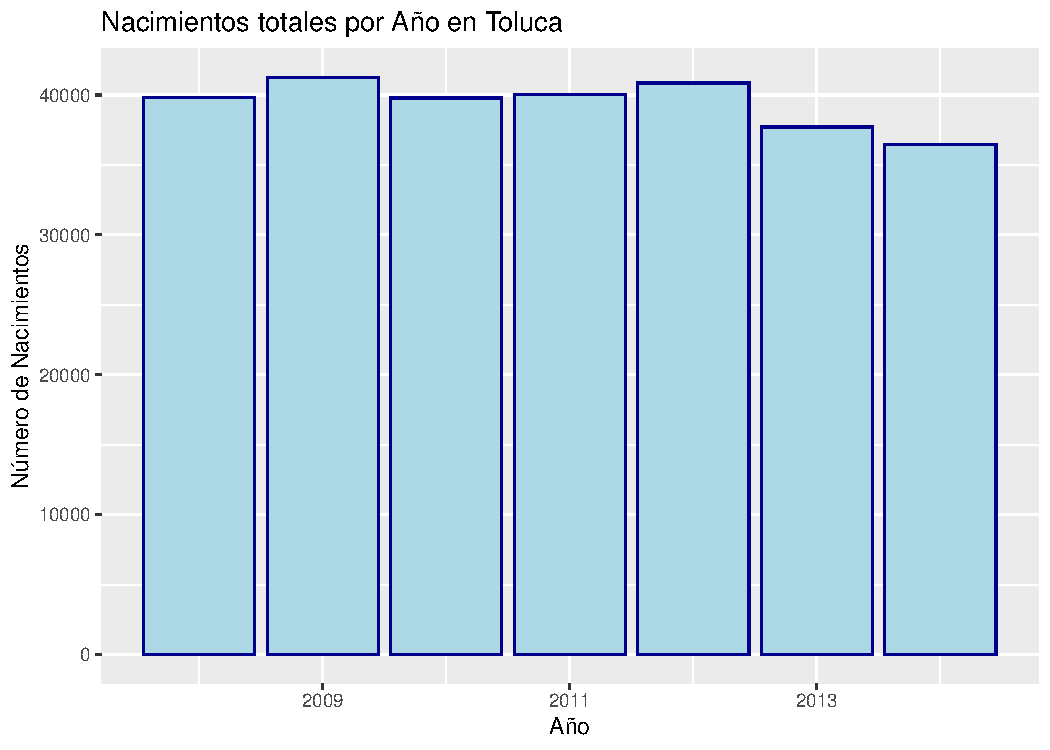
\includegraphics{bebes_toluca_files/figure-latex/Grafica_superficie -1} \end{center}

\hypertarget{cuxe1lculo-de-los-nacimientos-a-nivel-toluca-total}{%
\subsection{Cálculo de los nacimientos a nivel Toluca
(Total)}\label{cuxe1lculo-de-los-nacimientos-a-nivel-toluca-total}}

\begin{itemize}
\tightlist
\item
  Primero se calculó el promedio de nacimientos por año, que resultó:
  \textbf{39415}
\item
  Por lo que el promedio de nacimientos por mes fue: \textbf{3284.6}
\end{itemize}

\newpage

Ahora tenemos que análizar el numero de niños entre 0-2 años que hay por
cada AGEB en Toluca.

\begin{itemize}
\item
  Para ello obtenemos los totales por AGEB de Toluca, los comparamos con
  los nacimientos promedio y obtenemos el resultado aproximado.
\item
  Para ver los detalles del cálculo y manejo de datos puede consultar el
  código de R.
\end{itemize}

\begin{table}[H]
\centering\begin{table}[H]
\centering\begingroup\fontsize{8}{10}\selectfont

\resizebox{\linewidth}{!}{
\begin{tabular}{lc}
\toprule
AGEB & Número niños de 0 a 6 meses\\
\midrule
307 & 74.1\\
330 & 85.9\\
345 & 52.5\\
035A & 132.0\\
379 & 122.2\\
\addlinespace
383 & 52.0\\
398 & 36.3\\
400 & 49.1\\
415 & 38.8\\
042A & 51.5\\
\addlinespace
434 & 48.6\\
449 & 65.8\\
453 & 27.5\\
468 & 50.6\\
472 & 11.8\\
\addlinespace
487 & 54.5\\
491 & 43.2\\
504 & 61.3\\
519 & 16.2\\
523 & 46.1\\
\addlinespace
538 & 23.6\\
542 & 28.5\\
557 & 57.9\\
561 & 115.3\\
576 & 43.7\\
\addlinespace
580 & 10.3\\
595 & 20.6\\
608 & 50.6\\
631 & 48.6\\
646 & 132.5\\
\addlinespace
699 & 128.6\\
701 & 162.0\\
754 & 136.9\\
769 & 26.0\\
773 & 16.7\\
\addlinespace
788 & 121.7\\
824 & 29.9\\
858 & 131.0\\
862 & 263.6\\
896 & 208.6\\
\addlinespace
909 & 117.8\\
913 & 99.6\\
1023 & 72.1\\
1038 & 13.3\\
1061 & 85.4\\
\addlinespace
1254 & 83.9\\
1555 & 64.8\\
156A & 100.1\\
1606 & 55.0\\
1610 & 4.9\\
\addlinespace
1625 & 33.4\\
163A & 0.0\\
1663 & 29.0\\
1678 & 31.4\\
1682 & 132.0\\
\addlinespace
1697 & 20.1\\
1856 & 153.1\\
1860 & 132.0\\
188A & 114.8\\
1894 & 141.3\\
\addlinespace
1907 & 172.8\\
1911 & 105.0\\
1926 & 69.7\\
1930 & 89.8\\
1945 & 77.5\\
\addlinespace
195A & 74.6\\
1979 & 92.8\\
1983 & 176.2\\
1998 & 135.5\\
2017 & 110.9\\
\addlinespace
2021 & 76.1\\
2036 & 52.0\\
2040 & 91.3\\
2055 & 100.1\\
206A & 70.2\\
\addlinespace
2074 & 110.9\\
2089 & 75.1\\
2106 & 75.1\\
2110 & 41.7\\
2125 & 25.0\\
\addlinespace
213A & 34.8\\
2144 & 53.5\\
2159 & 26.5\\
2214 & 87.9\\
2248 & 80.0\\
\addlinespace
2290 & 20.6\\
2303 & 30.4\\
2318 & 29.9\\
2322 & 79.5\\
2337 & 52.0\\
\addlinespace
2341 & 33.4\\
2356 & 7.4\\
2360 & 36.8\\
2375 & 4.4\\
238A & 4.9\\
\addlinespace
2411 & 0.0\\
2426 & 25.0\\
2430 & 17.2\\
2445 & 58.4\\
245A & 61.8\\
\addlinespace
2572 & 146.7\\
2587 & 251.3\\
2604 & 30.4\\
2619 & 39.3\\
2623 & 144.3\\
\addlinespace
2638 & 80.5\\
2642 & 46.1\\
2657 & 19.1\\
2661 & 3.9\\
2676 & 47.1\\
\addlinespace
277A & 113.9\\
2799 & 31.9\\
2801 & 13.7\\
2816 & 31.4\\
3072 & 147.2\\
\addlinespace
3087 & 172.8\\
3091 & 78.0\\
3104 & 67.7\\
3119 & 133.5\\
3123 & 46.6\\
\addlinespace
3138 & 38.8\\
3142 & 117.8\\
3157 & 145.3\\
3161 & 47.6\\
3176 & 120.2\\
\addlinespace
3180 & 137.9\\
3195 & 52.5\\
3208 & 63.3\\
3212 & 46.6\\
3227 & 44.7\\
\addlinespace
3231 & 81.0\\
3246 & 49.1\\
3250 & 61.8\\
3265 & 25.0\\
327A & 177.7\\
\addlinespace
3284 & 134.0\\
3299 & 70.2\\
3301 & 160.5\\
3316 & 63.3\\
3320 & 90.8\\
\addlinespace
3335 & 94.2\\
334A & 87.4\\
3354 & 116.8\\
3369 & 106.0\\
3373 & 90.8\\
\addlinespace
3388 & 66.7\\
3392 & 11.3\\
3405 & 13.7\\
341A & 13.3\\
3424 & 10.3\\
\addlinespace
3496 & 121.7\\
3532 & 20.6\\
3547 & 24.0\\
3551 & 57.9\\
3566 & 53.5\\
\addlinespace
3570 & 39.8\\
3585 & 54.0\\
366A & 2.0\\
3674 & 2.5\\
3693 & 3.4\\
\addlinespace
3706 & 22.6\\
3710 & 82.5\\
3763 & 24.0\\
1729 & 162.5\\
1733 & 107.5\\
\addlinespace
2820 & 5.4\\
2962 & 11.3\\
359A & 12.8\\
1748 & 89.8\\
1752 & 109.4\\
\addlinespace
2765 & 20.6\\
2996 & 0.0\\
3000 & 2.5\\
1184 & 224.3\\
2708 & 14.2\\
\addlinespace
3015 & 6.4\\
3513 & 27.0\\
3636 & 22.1\\
2731 & 79.0\\
2746 & 122.2\\
\addlinespace
3655 & 173.3\\
1593 & 7.4\\
1767 & 194.4\\
1771 & 196.8\\
2407 & 49.1\\
\addlinespace
2680 & 52.0\\
2835 & 129.1\\
3602 & 3.9\\
241 & 120.7\\
284A & 2.5\\
\addlinespace
2977 & 52.0\\
2981 & 70.2\\
3458 & 20.6\\
3462 & 0.0\\
2500 & 121.7\\
\addlinespace
373A & 56.9\\
3744 & 121.2\\
1786 & 83.9\\
1790 & 125.2\\
2252 & 21.6\\
\addlinespace
302A & 7.4\\
3034 & 1.5\\
3477 & 6.9\\
2178 & 309.2\\
2854 & 71.2\\
\addlinespace
3049 & 30.4\\
3053 & 92.3\\
3068 & 194.8\\
3481 & 32.9\\
3689 & 49.6\\
\addlinespace
3725 & 69.7\\
294 & 189.0\\
1574 & 27.0\\
2750 & 10.8\\
2869 & 6.9\\
\addlinespace
2943 & 2.0\\
1485 & 80.5\\
149A & 66.7\\
2958 & 1.5\\
1502 & 250.8\\
\addlinespace
2271 & 168.8\\
2695 & 109.4\\
2873 & 75.1\\
2888 & 142.3\\
2182 & 235.6\\
\addlinespace
1517 & 218.9\\
1521 & 121.2\\
1589 & 82.9\\
1659 & 77.5\\
170A & 82.5\\
\addlinespace
2286 & 72.6\\
2394 & 5.4\\
2712 & 230.2\\
2727 & 230.2\\
2892 & 16.2\\
\addlinespace
1803 & 238.5\\
1818 & 199.3\\
2464 & 71.7\\
2553 & 11.8\\
2905 & 50.6\\
\addlinespace
3509 & 0.0\\
3528 & 0.0\\
3759 & 0.0\\
2479 & 136.0\\
3617 & 11.3\\
\addlinespace
1837 & 168.3\\
1841 & 286.1\\
2267 & 30.9\\
2515 & 120.2\\
2197 & 224.8\\
\addlinespace
2483 & 184.0\\
220A & 171.8\\
3621 & 16.2\\
252A & 117.3\\
2549 & 133.5\\
\addlinespace
3778 & 122.2\\
\bottomrule
\end{tabular}}
\endgroup{}
\end{table}
\end{table}

\end{document}
